\cleardoublepage

\chapter{Implementación}
\label{makereference5}



\section{Instalación y configuración del nodo principal}
\label{makereference5.1}
 Utilizando los repositorios de distribuciones oficiales de Sistemas operativos de Raspberry Pi, descargamos la versión ``Lite'' de Raspbian. Para establecer una conexión SSH por terminal es necesario crear un fichero con nombre \verb|ssh| en la raiz de la unidad de almacenamiento donde previamente se haya montado la imagen descargada. La distribución de Raspbian originalmente estaba configurada por defecto con la conexión de SSH abierta en el puerto 22, pudiendo accederse con el usuario \verb|pi| y la contraseña \verb|raspberry|. Este dato era ignorado por los usuarios menos experimentados y esto supuso una brecha de seguridad en todos las distribuciones que no fueron configuradas a posteriori por los usuarios según las indicaciones de la propia \href{https://www.raspberrypi.org/documentation/configuration/security.md}{documentación de Raspberry}~\cite{securingyourraspberrypi}. En el primer arranque del SO de la Raspberry se establecerán las configuraciones básicas para las sucesivas conexiones SSH basadas en autenticación con claves privadas.

 fiware citas bitpex

 De las estrategias disponibles para esta configuración, se crearán las claves en el equipo remoto que se conectará a la Raspberry, entregando mediante la primera conexión SSH con terminal la clave pública y almacenando la clave privada en el equipo remoto, reduciendo así el riesgo de ser expuesta fuera del dominio local del equipo. Para disponer de flexibilidad de conexión independientemente del SO del equipo remoto, la clave privada tendra un formato OpenSSH, fácil de incluir en SO Windows ya sea mediante conversión de la clave a formato PPK o como fichero accesible para aplicaciones de desarrollo, transferencias de ficheros, y/o control de versiones que integran conexiones SSH configurables (GitHub, Filezilla, Eclipse, etc). Los pasos necesarios para establecer conexiones cifradas robustas pueden encontrarse en el Anexo A seccion de implementación del Gateway.

Establecemos la capacidad de la Raspberry Pi 3 para su módulo de comunicación wifi de actuar como punto de acceso en modo NAT~\cite{raspberrypiasaccesspoint}. Se configura una red con acceso vía usuario y contraseña, con WPA2 y gestión de claves WPA-PSK. De esta forma, el nodo será capaz de desplegar una red inalámbrica que permitirá a otros dispositivos incorporarse a la suite domótica.

Descargamos la paquetería de Adafruit para el primer sensor de pruebas, el sensor DTH11 de temperatura y humedad.
Se requiere un montaje sencillo.
\begin{figure}[hbt!]
\centering
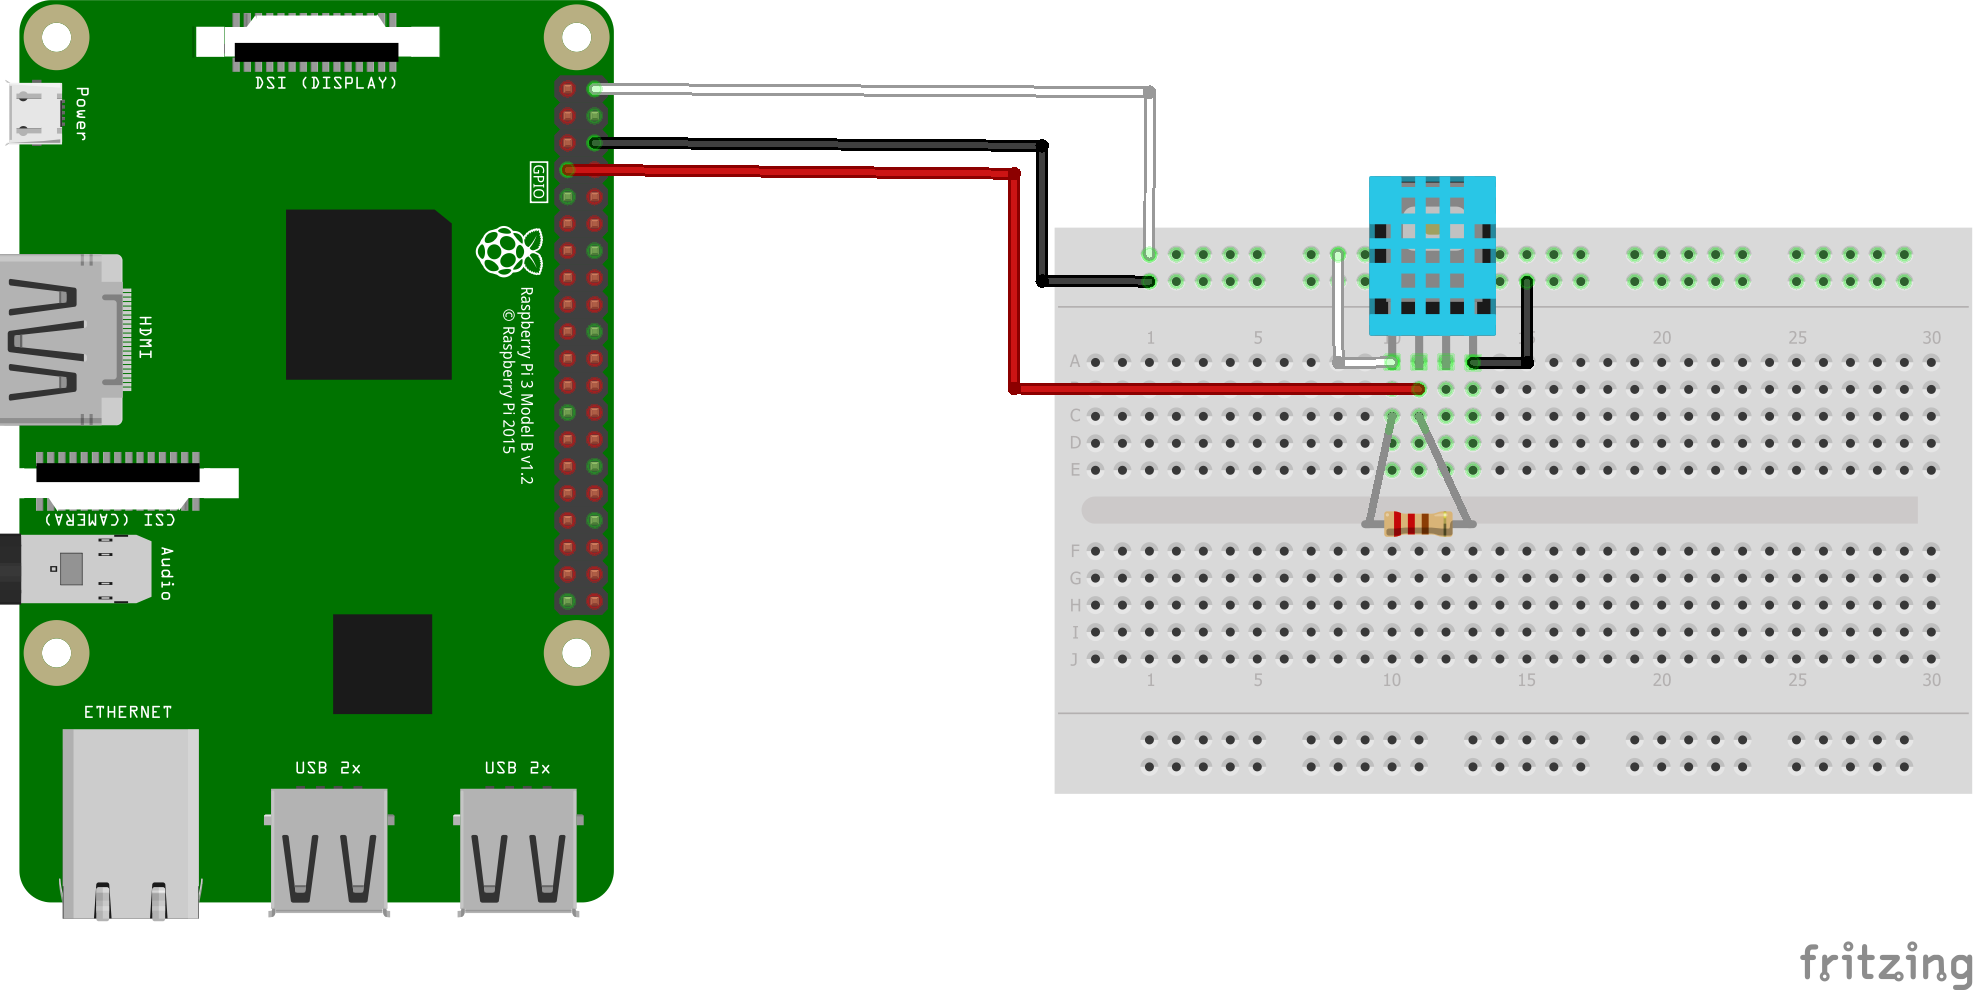
\includegraphics[height=2.5in]{figures/nodo_1.png}
\end{figure}

Clonamos la librería del sensor, nos ubicamos en la ruta descargada \verb|cd Adafruit_Python_DHT| e instalamos la librería \verb|sudo python setup.py install|, previamente instalamos las dependencias de la librería para su instalación \verb|sudo apt-get install python-setuptools| considerando que tenemos la versión de python 2.7.3, esto permitirá instalar la librería de python para el sensor DHT version 1.4. Se debe realizar una prueba de contacto con un script que nos muestre la información por pantalla para verificar que las conexiones del sensor a la rapsberry son correctos. Este primer script es un bucle infinito de mediciones de temperatura y humedad cada poco segundos. Hay una justificación para elegir un bucle sobre una única medida del sensor y está fundamentada en el margen de error inicial de las medidas. Si bien el sensor DTH11 es una opción muy común por su bajo coste y facilidad de implementación (este sensor se caracteriza por tener la señal digital calibrada por lo que asegura una alta calidad y una fiabilidad a lo largo del tiempo, ya que contiene un microcontrolador de 8 bits integrado. Está constituido por dos sensores resistivos (NTC y humedad) - revisar esta info y contrastarla contra ésta: \url{ https://programarfacil.com/blog/arduino-blog/sensor-dht11-temperatura-humedad-arduino/}), ademas de manejar señales digitales que no se ven afectadas por las fluctuaciones de voltaje, tiene algunas contrapartidas que deben tenerse en cuenta. Se necesita un tiempo mínimo de espera entre medidas (de al menos 1 segundo), hecho que no agrava particularmente su desempeño en entornos cerrados como una casa, ya que las variaciones de temperatura y humedad no son bruscas, aun así existen estrategias para reducir estos tiempos, por ejemplo, usar la función millis() de Arduino, el cual nos da el tiempo en milisegundos desde que empieza a ejecutarse el código, De esta forma evitamos la pausa de los 2 segundos, pero no el tiempo que demora en hacer la lectura, que es de aproximadamente  250 milisegundos, el cual lo pueden notar si realizan el ejemplo anterior, en donde se hace parpadear el led interno de la placa (Pin 13) con pausas de 100ms (tomado de \url{https://naylampmechatronics.com/blog/40_Tutorial-sensor-de-temperatura-y-humedad-DHT1.html}). Otro problema que abordar es que las primeras lecturas tienen un margen de error de unos +-2 grados Celsius y +-5\% de humedad relativa en las primeras 4 lecturas. Esto generará un problema a la hora de tomar lecturas instantáneas si el sensor no se encuentra ya operando cuando se solicita el dato. Como estrategia, haremos que el sensor tome medidas indefinidamente y los vuelque en un fichero/BBDD para recortar los tiempo de respuesta, evitando así esperar a que el sensor haga la toma de medidas en el momento+ de solicitud y sacándolas en su lugar del último registro que tengamos. Un último problema con el que hay que lidiar es su baja precisión limitada a enteros, por lo que no podemos esperar obtener un dato preciso a la décima de la temperatura y humedad. Esto sin embargo no es un problema real dada la naturaleza del proyecto, ya que no necesitamos un grado de precisión menor a la unidad para tomar acciones o informar al usuario.

En orden de subir sketcs a una arduino desde una Raspeberry Pi, es necesario isntalar las paqueterias del compilardor \verb|sudo apt-get install arduino-mk|, tras la instalación, en la ruta \verb|/usr/sahre/arduino| pueden encontrar binarios y una capeta llamada \verb|examples| que permiten cargan sketchs inmediatamente para comprobar el correcto funcionamiento del la placa microcontroladora. Para compilar dicho sketcs se necesita referenciar el fichero arduino.mk. De los ejemplo podemos verificar rampidamente el correcto funcionamiento de la microcontroladores utilizamos el mas basico de los sketcs, situado en \verb|/usr/share/arduino/examples/01.Basic/Blink/Blink.ino|, este ejemplo es muy basico, un loop que enciende y apaga el led integrado en la placa microcontroladora cada 1000 milisegundos. Este , es por defecto el sketch que generelamente los disitntos fabricantes de placas microcontroladoras de con procesador ATmega328P suelen dejar cargado a modo de test. Alterando el valor basico de sleep entre lineas de encendido y apagado a un valor menor como 50 milisegundos se puede comprobar si la comunicación del puerto com, y el compilador suben correctamente el codigo a la placa. Es importante verificar este punto antes de continuar y esta simple prueba cofirma que la configuración actual esta bien.

Para facilitar el proceso de subida de codigo a la placa de arduino, crearemos un Makefile hijo que enlace parametros al compilador.


Ahoera bien, tengamos en cuenta que las especificaciones del modulo esp8266 de wifi conectado a arduino requieren de una laimentación de 3.3V que pueden ser suministrados por la placa microcontroladora, sin embargo, esto nos deja con un problema de intensidad en la alimentación del modulo, ya que el pin de 3.3V disponible en la placa posees un amperaje de 50mA y se requieren de unos 200mA para garatizar una comunicación estable.
